\chapter{User-Guide\label{chap4:Viertes-Kapitel}}

Im folgenden Kapitel wird ein Überblick über alle implementierten Funktionalitäten aufgezeigt. So dient folgendes Kapitel auch als eine Art \glqq User-Guide\grqq{}.

\section{Login-/Logout-/Nutzerverwaltung\label{sec4.1:Unterpunkt-1}}

\begin{figure}[H]
    \centering
    \begin{minipage}{.4\textwidth}
        \begin{center}
            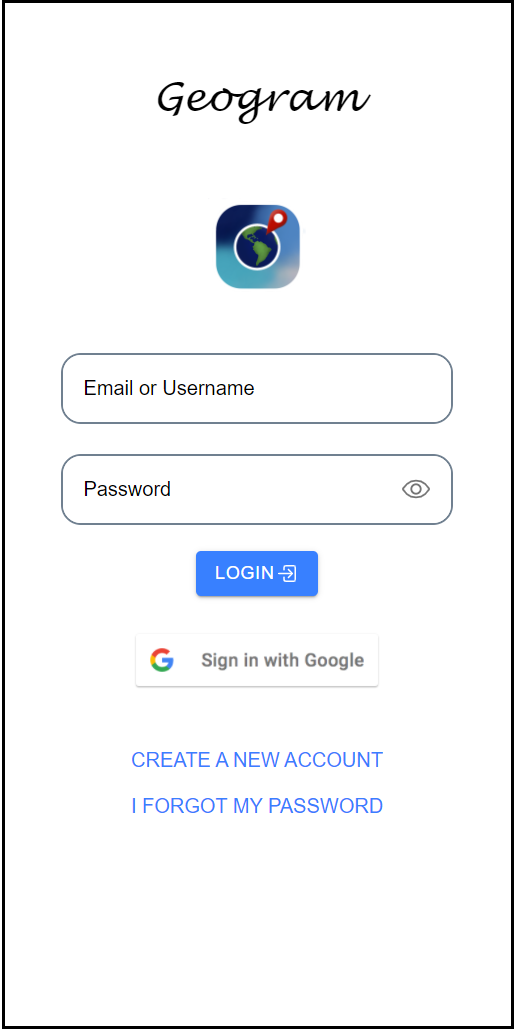
\includegraphics[width=0.8\linewidth]{images/Login.png}
        \end{center}
        \caption{Login - Ansicht}
        \label{fig:login}
    \end{minipage}%
    \begin{minipage}{.6\textwidth}
        \begin{changemargin}{0.5cm}{0cm}            
        Für den Anmeldevorgang benötigt der Besucher ein gültigen Account. Für die eigentliche Anmeldung wird das Passwort mit entweder der E-Mail-Adresse oder dem Usernamen benötigt. Zudem besteht auch die Möglichkeit sich mit einem Google-Account anzumelden.
        
        Sind die angegebenen Anmeldeinformationen nicht korrekt wird dem Besucher ein PopUp mit der Nachricht \glqq \textbf{Your Login credentials are incorrect}\grqq{} angezeigt.

        Neben dem Anmelden kann man über diese Ansicht noch die Funktionalitäten \glqq \textbf{Registrierung}\grqq{} und \glqq \textbf{Password vergessen}\grqq{} aufrufen.
        \end{changemargin}
    \end{minipage}
\end{figure}

\begin{figure}[H]
    \centering
    \begin{minipage}{.4\textwidth}
        \begin{center}
            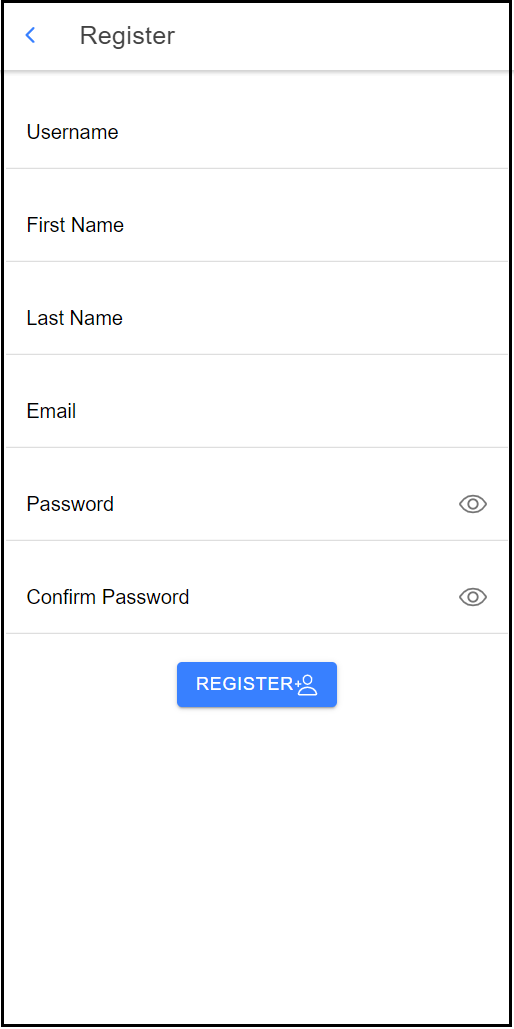
\includegraphics[width=0.8\linewidth]{images/Register.png}
        \end{center}
        \caption{Registrierungs - Ansicht}
        \label{fig:register}
    \end{minipage}%
    \begin{minipage}{.6\textwidth}
        \begin{changemargin}{0.5cm}{0cm}            
            Betätigt man auf der Login-Ansicht den Button \glqq \textbf{CREATE A NEW ACCOUNT}\grqq{}, so gelangt man auf die Registrierungs-Ansicht. Für einen neuen Account benötigt man folgende Informationen:

            \begin{itemize}
                \item \textbf{Username}
                \item \textbf{Vorname}
                \item \textbf{Nachname}
                \item \textbf{E-Mail}
                \item \textbf{Passwort}
            \end{itemize}

            Das Passwort muss folgende Bedingungen erfüllen:
            \begin{itemize}
                \item \textbf{Mindestens 6 Zeichen lang}
                \item \textbf{mind. eine Zahl}
                \item \textbf{mind. ein Sonderzeichen}
            \end{itemize}
        \end{changemargin}
    \end{minipage}
\end{figure}

\begin{figure}[H]
    \centering
    \begin{minipage}{.4\textwidth}
        \begin{center}
            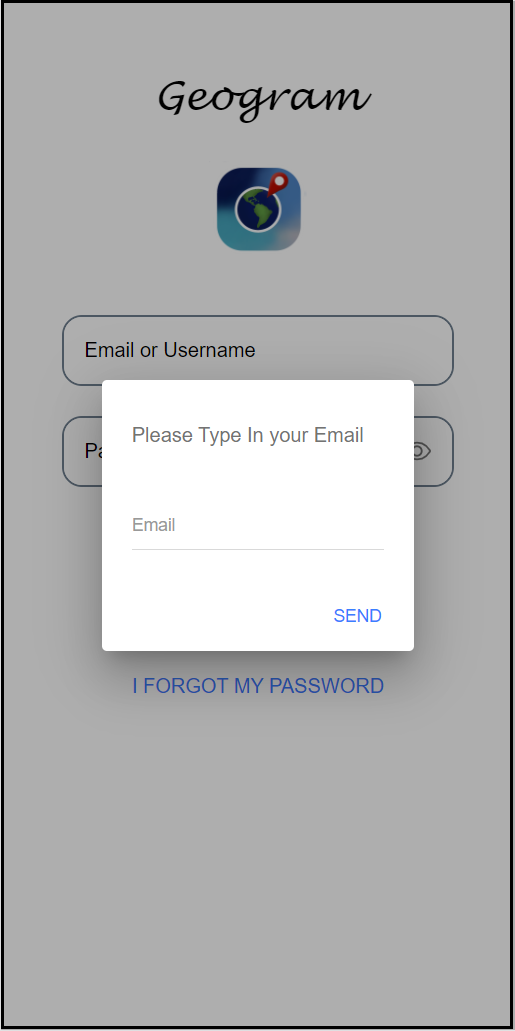
\includegraphics[width=0.8\linewidth]{images/forgetemail.png}
        \end{center}
        \caption{E-Mail-Vergessen - Ansicht}
        \label{fig:forgetemail}
    \end{minipage}%
    \begin{minipage}{.6\textwidth}
        \begin{changemargin}{0.5cm}{0cm}            
            Falls der Besucher sein Password für seinen Account vergessen hat, so kann er mit der \glqq Password-Vergessen\grqq{}-Funktionalität ein neues Password hinterlegen. Hierfür muss er seine gültige Account-E-Mail angeben und erhält von Geogram eine E-Mail zugesendet. In dieser E-Mail befindet sich ein Link, mit welchem der Besucher seinem Account ein neues Password hinterlegen kann.
        \end{changemargin}
    \end{minipage}
\end{figure}

\section{Profil - Ansicht\label{sec4.2:Unterpunkt-2}}

\begin{figure}[H]
    \centering
    \begin{minipage}{.4\textwidth}
        \begin{center}
            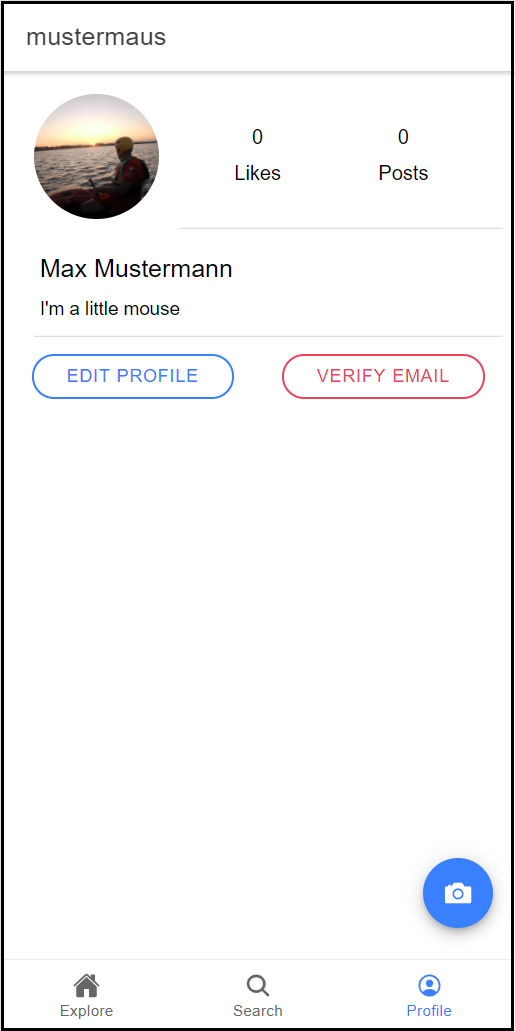
\includegraphics[width=0.8\linewidth]{images/profil.png}
        \end{center}
        \caption{Profil - Ansicht}
        \label{fig:profil}
    \end{minipage}%
    \begin{minipage}{.6\textwidth}
        \begin{changemargin}{0.5cm}{0cm}            
            In der Profil-Ansicht hat der Benutzer die Möglichkeit Informationen über sein eigenes Profil zu sehen.

            Zu sehen sind folgende Informationen:
            \begin{itemize}
                \item \textbf{Profilbild}
                \item \textbf{Anzahl erhaltener Likes}
                \item \textbf{Anzahl veröffentlichter Posts}
                \item \textbf{Vor- und Nachname}
                \item \textbf{Biographie (Text über sich selbst)}
                \item \textbf{Die eigenen Posts}
            \end{itemize}

            Zusätzlich hat man noch die Möglichkeit folgende Funktionalitäten auf der Profil-Ansicht auszuführen:
            \begin{itemize}
                \item \textbf{Ändern des Profilbildes (Durch drücken des Bildes)}
                \item \textbf{Profil bearbeiten}
                \item \textbf{Einmalige Verifizierung der E-Mail}
            \end{itemize}
        \end{changemargin}
    \end{minipage}
\end{figure}

Mit drücken eines Posts öffnet sich das PopUp aus \autoref{fig:post_popup}, über welches man auf die Post-Info aus \autoref{fig:post_info} gelangt.

\begin{figure}[H]
    \centering
    \begin{minipage}{.5\textwidth}
      \centering
      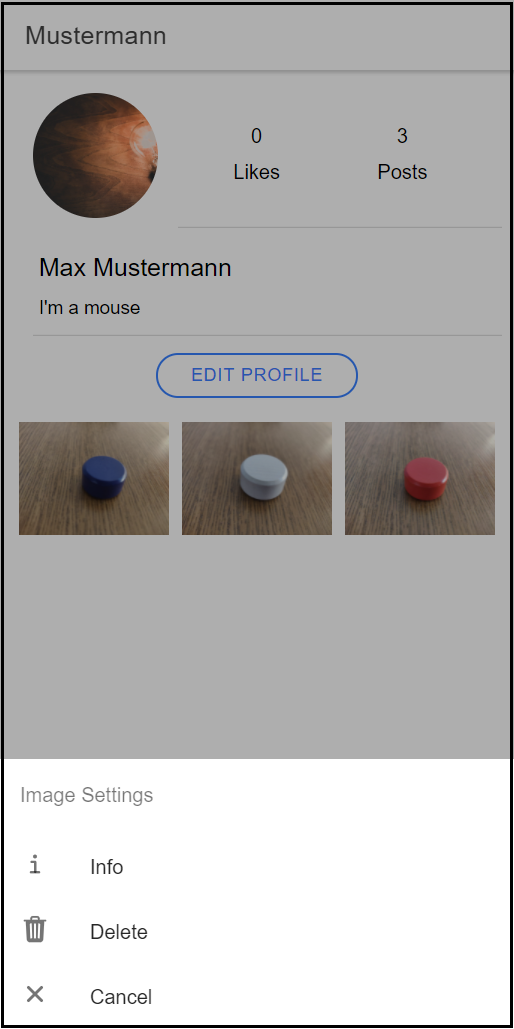
\includegraphics[width=.6\linewidth]{images/post_popup.png}
      \caption{Post-PopUp}
      \label{fig:post_popup}
    \end{minipage}%
    \begin{minipage}{.5\textwidth}
      \centering
      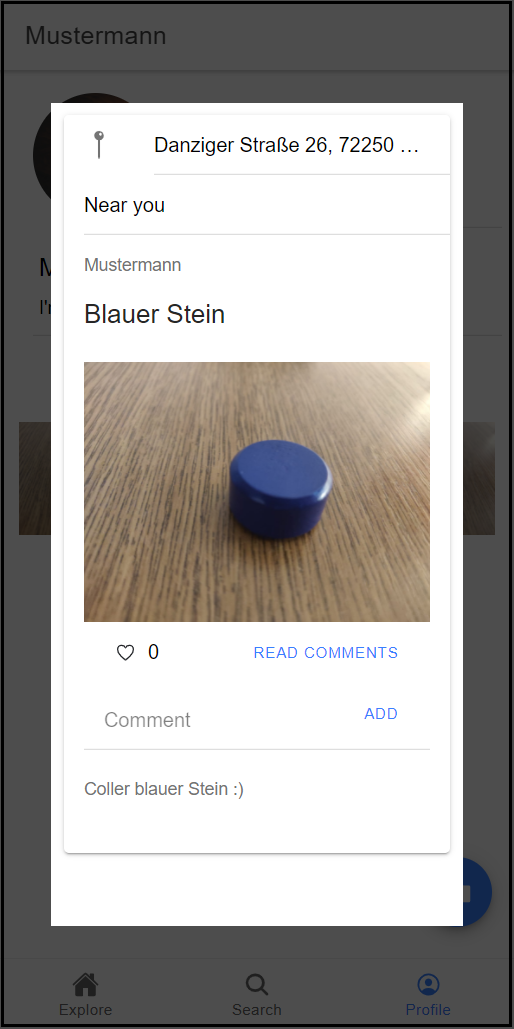
\includegraphics[width=.6\linewidth]{images/post_info.png}
      \caption{Post Informationen}
      \label{fig:post_info}
    \end{minipage}
\end{figure}

\begin{figure}[H]
    \centering
    \begin{minipage}{.4\textwidth}
        \begin{center}
            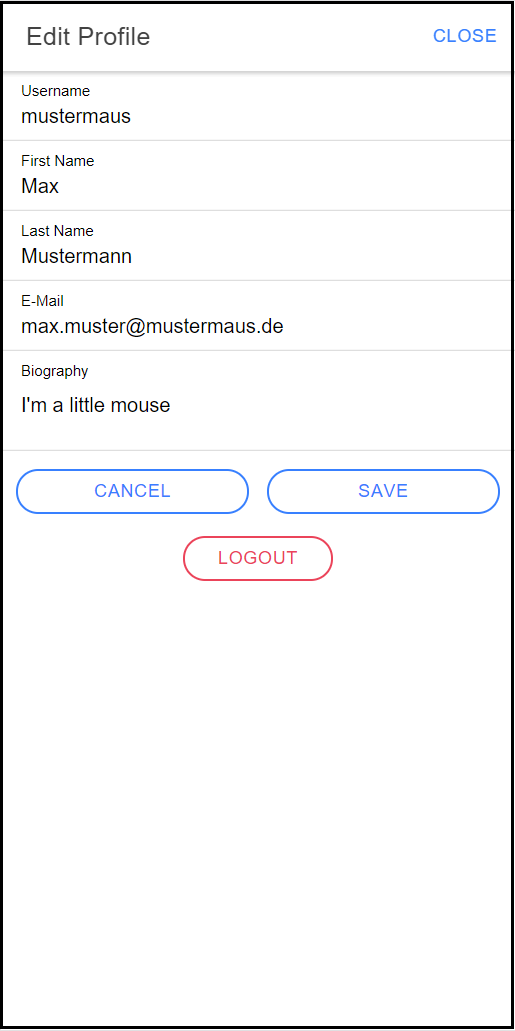
\includegraphics[width=0.8\linewidth]{images/editProfil.png}
        \end{center}
        \caption{Edit Profil - Ansicht}
        \label{fig:editprofil}
    \end{minipage}%
    \begin{minipage}{.6\textwidth}
        \begin{changemargin}{0.5cm}{0cm}            
            In dieser Ansicht hat der Benutzer zusätzlich die Möglichkeit die Informationen des Profils zu überarbeiten.

            Bearbeitet werden können folgende Informationen:
            \begin{itemize}
                \item \textbf{Benutzername}
                \item \textbf{Vorname}
                \item \textbf{Nachname}
                \item \textbf{E-Mail}
                \item \textbf{Biographie (Text über sich selbst)}
            \end{itemize}

            Zusätzlich hat man hier die Möglichkeit sich von Geogram abzumelden. Man gelangt dann wieder zur Login-Ansicht.
        \end{changemargin}
    \end{minipage}
\end{figure}

\section{Suchen - Ansicht\label{sec4.3:Unterpunkt-3}}

\begin{figure}[H]
    \centering
    \begin{minipage}{.4\textwidth}
        \begin{center}
            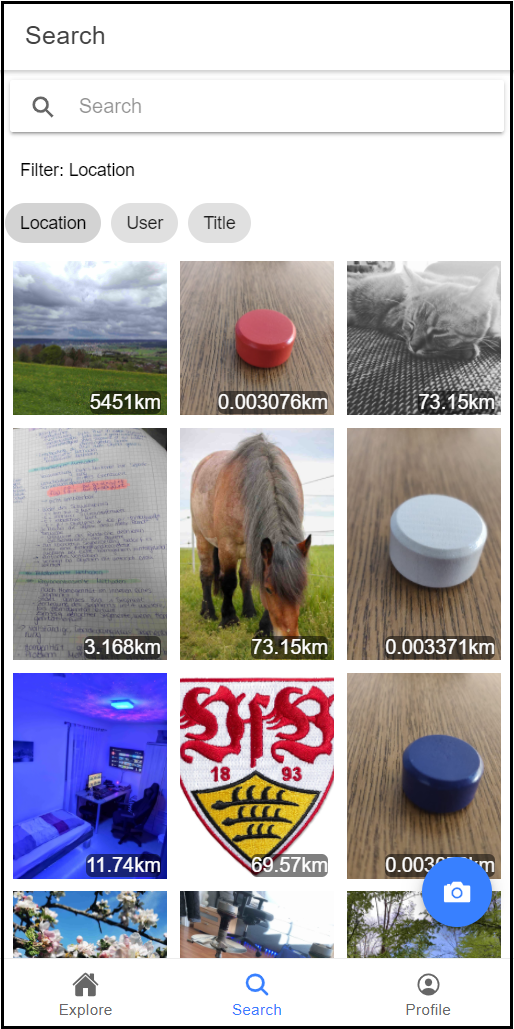
\includegraphics[width=0.8\linewidth]{images/Search.png}
        \end{center}
        \caption{Suchen - Ansicht}
        \label{fig:searchTab}
    \end{minipage}%
    \begin{minipage}{.6\textwidth}
        \begin{changemargin}{0.5cm}{0cm}            
            Mit dem Tab \glqq \textbf{Search}\grqq{} gelangt der Benutzer auf die nebenstehende Ansicht. Hier hat der Benutzer die Möglichkeit nach bestimmten Posts zu suchen.

            Bei den einzelnen Posts werden jeweils die Bilder und die dazugehörigen Entfernungen zum Benutzer angezeigt und erst beim Drücken eines Posts erhält man eine Info-Ansicht, wie aus \autoref{fig:post_info}.

            Zu Beginn werden alle verfügbaren Posts angezeigt. Der Benutzer hat jedoch auch die Möglichkeit die angezeigten Posts zu filtern. Gefiltert werden kann nach der Entfernung, dem User oder dem Titel.
        \end{changemargin}
    \end{minipage}
\end{figure}

\section{Explore - Ansicht\label{sec4.4:Unterpunkt-4}}

\begin{figure}[H]
    \centering
    \begin{minipage}{.4\textwidth}
        \begin{center}
            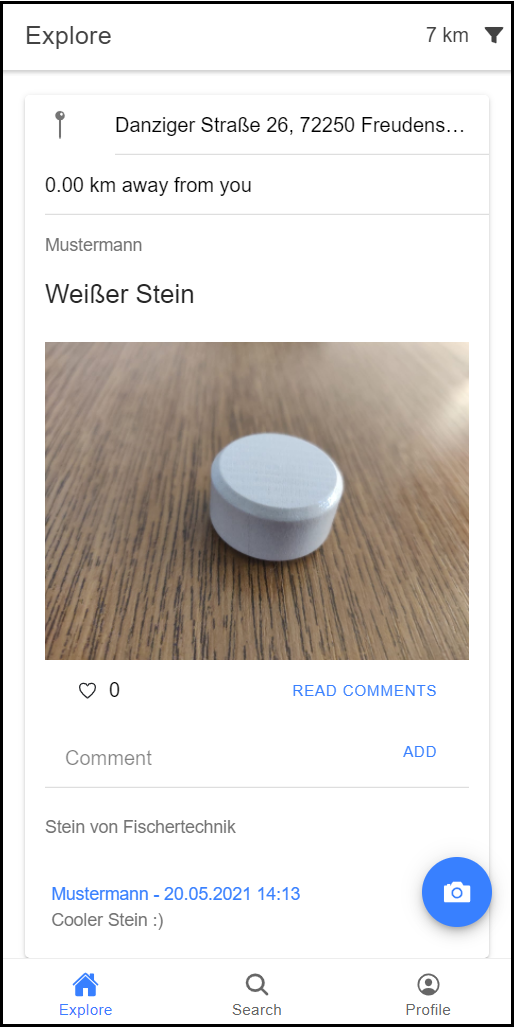
\includegraphics[width=0.8\linewidth]{images/explore.png}
        \end{center}
        \caption{Explore - Ansicht}
        \label{fig:exploreTab}
    \end{minipage}%
    \begin{minipage}{.6\textwidth}
        \begin{changemargin}{0.5cm}{0cm}            
            Mit dem Tab \glqq \textbf{Explore}\grqq{} gelangt der Benutzer auf die nebenstehende Ansicht. Hier werden dem Benutzer die vollständigen Posts angezeigt.

            Dem Benutzer werden die Posts abhängig von der Entfernung entweder angezeigt oder nicht. Um den Radius der Entfernung zu ändern, kann der Benutzer diesen oben rechts einstellen. Wird der Radius auf \glqq \textbf{30+}\grqq{} gestellt, so werden alle Posts angezeigt.

            Bei jedem Post hat der Benutzer die Möglichkeit ein Like und Kommentare abzugeben. Den eigenen Kommentar und die Kommentare von anderen Benutzern kann man ebenfalls unter den Posts sehen. 
        \end{changemargin}
    \end{minipage}
\end{figure}
